\documentclass{segabs}
\usepackage{amsmath}
\usepackage{algorithm}
\usepackage{algorithmic} 
\usepackage{mathtools}
\graphicspath{ {images/} }
\DeclarePairedDelimiter{\ceil}{\lceil}{\rceil}

\newcommand{\truegamma}{\gamma_*}
\newcommand{\deltagamma}{{\Delta\gamma}}
\newcommand{\deltagammaguess}{{\widetilde{\deltagamma}}}
\newcommand{\Done}{{\mathcal{D}_1}}
\newcommand{\Dtwo}{{\mathcal{D}_2}}
\newcommand{\undermedian}[2]{\underset{#1}{\text{median}}\,\,\,#2}
\newcommand{\scalefactor}{\ln \left(\sqrt{\frac{t_c}{t_b}\cdot\frac{t_d}{t_a}} \,\right) } 
\newcommand{\rateofconvergence}{ \frac{\ln \left(\frac{t_b}{t_c}\cdot \frac{t_d}{t_a} \right)}{\ln \left(\frac{t_c}{t_b}\cdot \frac{t_d}{t_a} \right)}}
\newcommand{\Drightabove}{{\mathcal{D}_{rt,abv}}}
\newcommand{\Dleftbelow}{{\mathcal{D}_{lt,blw}}}
\newcommand{\Dbelow}{{\mathcal{D}_{blw}}}
\newcommand{\tcut}{t_{cut,abv}}
\newcommand{\tcutbelow}{t_{cut,blw}}

\begin{document}

\title{Median balancing: A linearly convergent algorithm for time gain power correction }

\renewcommand{\thefootnote}{\fnsymbol{footnote}} 

\author{Yenming Lai\footnotemark[1], Eric Price, Rachel Ward, 
  and Sergey Fomel, University of Texas at Austin}

\footer{Example}
\lefthead{Lai, Price, Ward \& Fomel}
\righthead{Median balancing}

\maketitle

\begin{abstract}
Time-power gain is an important step in seismic data processing. In 1985, Jon Claerbout and Zhiming Li suggested in a single-page report a simple algorithm to estimate automatic time gain correction in the observed data. We prove that their algorithm with a minor modification converges linearly under the single assumption that the median in the first half of the absolute value of the corrected signal is equal to the median in the second half of the absolute value of the signal. Furthermore, we derive a guaranteed rate of convergence and show the error penalty on convergence rate when the assumption does not hold.  To use the algorithm, the user is required only to specify a desired tolerance from the true gain correction power and, optionally, an initial guess of the gain correction power. The initial guess does not affect the convergence guarantee, only the number of iterations needed for convergence. The algorithm is tested successfully against field data.  
\end{abstract}

\section{Introduction}

Field seismic data commonly suffer from amplitude attenuation.  A simple but common method to correct this attenuation is to apply a time power gain $t^\gamma$ where the power $\gamma$ is a fixed constant. \cite{o1971reflections} suggest $\gamma=3/2$. \cite{Fowler.sep.38.73} and \cite{iei} suggest $\gamma=2$, one power of $t$ for spherical divergence and another power for attenuation. In actual seismic traces, however, $\gamma$ may vary. 

The power law for frequency rather than time is commonly used to describe fractal behavior of sedimentary rocks \cite[]{Walden_H85,Hewett_86,Stefani_G01,Anstey_D02a,Anstey_D02b}. The power law constant can be measured by analyzing frequency spectra of well logs \cite[]{browaeys2009fractal}.

\cite{Fowler.sep.38.73} develop an algorithm for $\gamma$ estimation based on maximizing a semblance-like objective function. \cite{Claerbout.sep.42.81} propose a simpler iterative algorithm based on median balancing and report its fast convergence. The algorithm divides the absolute value of the signal into two time windows and finds the time power constant that balances the medians of the two time windows. 

In this paper, we modify the median balancing algorithm to improve its behavior and formally prove the algorithm's convergence. We show that the convergence rate is at worst linear. We test the modified algorithm on data examples.

\section*{Problem Setup}

Let $c[t]$ be the correct, unattenuated discrete signal which is attenuated by some fixed time power $\gamma > 0$. Then, $d[t]$, the observed signal, can be written as 

\begin{equation}
\label{eqn:d}
d[t] = t^{-\gamma} c[t] 
\end{equation}   

We use the square bracket notation to indicate that the time values are discrete. Our goal is to recover $\gamma$ and, by doing so, to recover $c[t]$ given $d[t]$.  

Suppose the observed signal $d[t]$ is of length $N$ and takes on values at time values $\mathcal{D} = \{t_1,t_2,\ldots,t_N\}$ with  $t_1 < t_2 < \ldots < t_N$. Split the time values, the domain of $d[t]$, in half as follows: If $N$ is even, let $\mathcal{D}_1 = \{t_1, t_2,\ldots, t_\frac{N}{2} \}$ and $\mathcal{D}_2 = \{ t_{\frac{N}{2}+1},t_{\frac{N}{2}+2}, \ldots, t_N \}$. If $N$ is odd, let $\mathcal{D}_1 = \{t_1, t_2,\ldots, t_\frac{N+1}{2} \}$ and $\mathcal{D}_2 = \{ t_{\frac{N+1}{2}+1},t_{\frac{N}{2}+2}, \ldots, t_N \}$. Let the end points of $\mathcal{D}_1$ and $\mathcal{D}_2$ be given as $t_a=\min{\Done}, t_b=\max{\Done}$ and $t_c=\min{\Dtwo}, t_d=\max{\Dtwo}$ respectively.



\section*{Median Balancing Algorithm}


Algorithm \ref{euclid} gives the pseudo code for our median balancing algorithm, which is a slight modification of the original algorithm by \cite{Claerbout.sep.42.81}. 
\begin{algorithm}
\caption{Median Balancing}\label{euclid}
\begin{algorithmic} 
\STATE $\gamma = \gamma_0$
\STATE step\_size\_scaling = $\scalefactor$
\WHILE{$\deltagammaguess < \mbox{tolerance}$ }
\STATE $M_\Done = \undermedian{t\in \Done}{t^\gamma |d[t]|}$
\STATE $M_\Dtwo = \undermedian{t\in \Dtwo}{t^\gamma |d[t]|}$
\STATE $\deltagammaguess = \ln \left(\frac{M_\Done}{M_\Dtwo} \right) / \text{step\_size\_scaling}$
\STATE $\gamma = \gamma + \deltagammaguess$
\ENDWHILE
\end{algorithmic} 
\end{algorithm}

Our modification to Claerbout and Li's algorithm is setting the step size scaling factor to be $\scalefactor$ instead of the natural log ratio of the midpoints of $\Dtwo$ and $\Done$ e.g $\ln \frac{\frac{t_c+t_d}{2}}{\frac{t_b+t_a}{2}}$.  Our derivation shows that the modified step size  helps balance overstepping and understepping at each iteration.

\subsection{Assumption needed for linear convergence}

For the algorithm to converge linearly, we assume that the median in the first half of the absolute value of the signal is equal to the median in the second half of the absolute value of the signal, that is 

\begin{equation}
 \undermedian{t \in \Done}{ |c[t]| }  = \undermedian{t \in \Dtwo}{|c[t]|}  
\end{equation}


If $c[t]$ is a realization of signal with a fixed random distribution, then assumption 1 holds with high probability.

If we wish to find the correct time gain power correct $\gamma$ for a family of $M$ traces, that is $d[t,x]$ with $x \in \{n_1, n_2, \ldots, n_M\}$, we simply modify the algorithm's lines calculating $M_\Done$ and $M_\Dtwo$ to 


\begin{algorithmic} 
\STATE $M_\Done = \undermedian{t\in \Done, \,\, \mbox{all $x$}}{t^\gamma |d[t,x]|}$
\STATE $M_\Dtwo = \undermedian{t\in \Dtwo, \,\, \mbox{all $x$}}{t^\gamma |d[t,x]|}$
\end{algorithmic} 


Our assumption then becomes

\begin{equation}
 \undermedian{t\in \Done, \,\, \mbox{all $x$}}{ |c[t]| }  = \undermedian{t\in \Dtwo, \,\, \mbox{all $x$}}{|c[t]|}  
\end{equation}

\section*{Proof of linear convergence of median balancing algorithm}

We now show that our algorithm converges linearly to the true gamma $\truegamma$ and calculate a rate of convergence guarantee. We first derive a condition that implies linear convergence and then shows how this conditions implies linear convergence and a guaranteed rate of convergence.

%\subsection{Derivation of condition implying linear convergence}

Let $d_{\gamma}[t]$ be the absolute value of $d[t]$ corrected by some \emph{guess} at the time power $\gamma$, that is

\begin{equation}
\label{eqn:d_gamma}
d_\gamma[t] = t^\gamma \left| d[t] \right|
\end{equation}

with $t \in \mathcal{D}$.  Let the difference between $\gamma$ and the true gamma $\truegamma$ be denoted as 

\begin{equation}
\label{eq:deltagamma_def}
\deltagamma = \truegamma - \gamma
\end{equation}

By substituting (\ref{eqn:d}) into (\ref{eqn:d_gamma}) and rearranging terms, we have

\begin{equation}
|c[t]|=t^{\deltagamma} d_\gamma[t]
\end{equation}  

In other words, the correct signal is the $\gamma$ corrected signal, $d_\gamma$, with the additional correction of $t^{\deltagamma}$.  

Let the median value of the absolute value of the correct signal $c[t]$ in its left partition $\Done$ divided by the median value of the absolute value of the correct signal $c[t]$ in its right partition $\Dtwo$ be denoted as $\alpha$, that is  

\begin{equation}
\label{eq:alpha}
\alpha = \frac{\undermedian{t \in \Done}{ |c[t]| } }{\undermedian{t \in \Dtwo}{|c[t]|} } = \frac{\undermedian{t \in \Done}{t^\deltagamma d_\gamma[t]} }{\undermedian{t \in \Dtwo}{t^\deltagamma d_\gamma[t]} }
\end{equation}


Assume that $\deltagamma \geq 0$. The derivation in the case that $\deltagamma < 0$ is symmetric and arrives at the same linear convergence rate guarantee.  We wish to add both upper and lower bounds to both the numerator and the denominator of (\ref{eq:alpha}).  Hence, using the minimum and maximum values $\Done$ and $\Dtwo$ respectively, we have

\begin{equation}
\label{eq:alpha_num_bound}
 t_a^\deltagamma \undermedian{t \in \Done}{ d_\gamma[t]}  \leq \undermedian{t \in \Done}{t^\deltagamma d_\gamma[t]}  \leq t_b^\deltagamma \undermedian{t \in \Done}{ d_\gamma[t]} 
\end{equation}

and

\begin{equation}
\label{eq:alpha_den_bound}
 t_c^\deltagamma \undermedian{t \in \Done}{ d_\gamma[t]}  \leq \undermedian{t \in \Done}{t^\deltagamma d_\gamma[t]}  \leq t_d^\deltagamma \undermedian{t \in \Done}{ d_\gamma[t]} 
\end{equation}

Using (\ref{eq:alpha_num_bound}) and (\ref{eq:alpha_den_bound}), we bound (\ref{eq:alpha}) as follows

\begin{equation}
\label{eq:alpha_bounded}
\frac{t_a^\deltagamma\undermedian{t \in \Done}{ d_\gamma[t]} }{t_d^\deltagamma\undermedian{t \in \Dtwo}{ d_\gamma[t]} }\leq \underbrace{ \frac{\undermedian{t \in \Done}{t^\deltagamma d_\gamma[t]} }{\undermedian{t \in \Dtwo}{t^\deltagamma d_\gamma[t]} }}_\alpha \leq
\frac{t_b^\deltagamma\undermedian{t \in \Done}{ d_\gamma[t]} }{t_c^\deltagamma\undermedian{t \in \Dtwo}{ d_\gamma[t]} }
\end{equation}

Taking the natural logarithm of all three terms in (\ref{eq:alpha_bounded}) and rearranging terms, we arrive at

\begin{equation}
\label{eq:alpha_bounded_two}
\ln \alpha + \ln \frac{t_c}{t_b}  \deltagamma \leq \ln \frac{\undermedian{t \in \Done}{ d_\gamma[t]}}{\undermedian{t \in \Dtwo}{ d_\gamma[t]}} \leq \ln \alpha + \ln \frac{t_d}{t_a} \deltagamma 
\end{equation}

Divide all terms of (\ref{eq:alpha_bounded_two}) by the natural log of the geometric mean of the partition end point ratios $\frac{t_c}{t_b}$ and $\frac{t_d}{t_a}$, that is the constant scaling factor $\scalefactor$, to get

\begin{eqnarray}
\label{eq:alpha_bounded_three}
\frac{\ln \alpha}{\scalefactor} + \frac{\ln \frac{t_c}{t_b}\deltagamma }{\scalefactor} & \leq & \underbrace{ \frac{\ln \frac{\undermedian{t \in \Done}{ d_\gamma[t]}}{\undermedian{t \in \Dtwo}{ d_\gamma[t]}} }{\scalefactor}}_{\equiv \deltagammaguess} \nonumber \\ 
& \leq & \frac{\ln \alpha}{\scalefactor} + \frac{\ln \frac{t_d}{t_a}\deltagamma }{\scalefactor} \nonumber \\
\end{eqnarray}

If the median value of $c[t]$ in its left partition is equal to the median value of $c[t]$ in its right partition, that is $\alpha=1$, the pair of inequalities of (\ref{eq:alpha_bounded_three}) simplifies to 

\begin{equation}
\label{eq:alpha_bounded_four}
 \frac{\ln\frac{t_c}{t_b}}{\scalefactor} \deltagamma \leq \deltagammaguess \leq \frac{\ln\frac{t_d}{t_a}}{\scalefactor} \deltagamma
\end{equation}

%\subsection{Condition (\ref{eq:alpha_bounded_four}) implies linear convergence}

We now show that (\ref{eq:alpha_bounded_four}) implies linear convergence and calculate the guaranteed rate of convergence $\mu \in (0,1)$.  Let $\gamma$ at iteration $n$ be defined as $\gamma_n$. As before, $\truegamma$ is the true gamma.  Let

\begin{equation}
\deltagamma_n =\truegamma - \gamma_n,
\end{equation}

and let
\begin{equation}
\deltagammaguess_n = \frac{\ln \frac{\undermedian{t \in \Done}{t^{\deltagamma_n} d_{\gamma_n}[t]}}{\undermedian{t \in \Done}{t^{\deltagamma_n} d_{\gamma_n}[t]}} }{\scalefactor}
\end{equation}

We want to show that if the $n$-th iteration of (\ref{eq:alpha_bounded_four}) holds, that is  

\begin{equation}
\label{eq:linear_convergence_condition_n}
 \frac{\ln\frac{t_c}{t_b}}{\scalefactor} \deltagamma_n \leq \deltagammaguess_n \leq \frac{\ln\frac{t_d}{t_a}}{\scalefactor} \deltagamma_n\end{equation}


then we have linear convergence at rate \emph{slowest} $\mu \in (0,1)$, that is 

\begin{equation}
\frac{|\truegamma - \gamma_{n+1}|}{|\truegamma - \gamma_{n}|} \leq \mu \quad \quad \forall n 
\end{equation}

Adding and subtracting $\truegamma$ and letting $\deltagamma_n =\truegamma - \gamma_n$, we have
\begin{equation}
\label{eq:gamma_n}
\gamma_n = \gamma_n - \truegamma + \truegamma = -\deltagamma_n + \truegamma
\end{equation}

From our algorithm, we have
\begin{equation}
\label{eq:gamma_n_1}
\gamma_{n+1} = \gamma_n + \deltagammaguess_n
\end{equation}

Substituting (\ref{eq:gamma_n}) into (\ref{eq:gamma_n_1}) and rearranging terms gives

\begin{equation}
\label{eq:truegamma_gamma_n_1}
\truegamma - \gamma_{n+1} = \deltagamma_n - \deltagammaguess_n
\end{equation}

Subtracting $\deltagamma_n$ from all three terms of (\ref{eq:linear_convergence_condition_n}) implies

\begin{equation}
\label{eq:deltagamma_deltagamma_n_1}
|\deltagamma_n - \deltagammaguess_n| \leq \rateofconvergence |\underbrace{\deltagamma_n}_{\truegamma - \gamma_n}|
\end{equation}

We note that the derivation in the case $\deltagamma <0$ arrives at equation (\ref{eq:deltagamma_deltagamma_n_1}) also.   Taking the absolute value of (\ref{eq:truegamma_gamma_n_1}) and using (\ref{eq:deltagamma_deltagamma_n_1}), we then have, as desired,

\begin{equation}
\label{eq:convergence_rate}
\frac{|\truegamma - \gamma_{n+1}|}{|\truegamma - \gamma_{n}|} \leq \rateofconvergence = \mu
\end{equation}

\subsection{Convergence rate if assumption does not hold}

If  assumption 1 does not hold, then $ \undermedian{t \in \Done}{ |c[t]| }  \neq \undermedian{t \in \Dtwo}{|c[t]|}  
$ and hence $\alpha \neq 1$. Beginning with (\ref{eq:alpha_bounded_three}) instead of (\ref{eq:alpha_bounded_four}), we follow a parallel derivation as the previous section by carrying the term $\frac{\ln \alpha}{\scalefactor}$ through the derivations and arrive at a new convergence rate $\mu_{err}$, that is 

\begin{equation}
\frac{|\truegamma - \gamma_{n+1}|}{|\truegamma - \gamma_{n}|} \leq \underbrace{\mu + |\frac{\ln \alpha}{\scalefactor}|}_{\mu_{err}}
\end{equation}

We note that with $\alpha \neq 1$ our algorithm is still guaranteed to converge but recovers a  $\gamma$ that is not exactly $\truegamma$.  By continuity and monotonicity of the function $t^{\gamma}$, there will always exist some "true" $\gamma$ at which  the medians are equal. Thus the algorithm will always converge to some $\gamma$.

\subsection{Faster rate of convergence observed in practice}

In practice, we observe a faster rate of convergence and thus a smaller $\mu$ than our theory guarantees.  For example, for a 4 second trace sampled every 0.002 seconds and beginning at time equal to 1 second, we have the partition end points $t_a=1, t_b=2.998, t_c=3, t_d =5$, which implies a guaranteed convergence rate of $\mu \approx 0.999$.

A smaller $\mu$ means either of the following conditions:

(1) The gap between $t_c$ and $t_b$ is large. 

(2) The gap between $t_d$ and $t_a$ is small.
   
The two conditions imply medians occur closer to the middle of the partition.  For example, if we have the partition end points $t_a=1.5, t_b=2.5, t_c=3.5, t_d =4.5$, we then have a guaranteed convergence rate of $\mu \approx 0.531$. Interestingly enough,  \cite{Claerbout.sep.42.81} assume implicitly that medians occur in the middle of the partition.

The convergence derivation relies essentially on the bounds of (\ref{eq:alpha_num_bound}) and (\ref{eq:alpha_den_bound}), and these bounds are tight. For example, let $d_\gamma[t]$ be a length 3 signal taking on the values  $1,\frac{1}{16},\frac{1}{4}$ at times $1,2,3$ respectively and let $\deltagamma=1$.  The median of $d_\gamma[t]$ is $\frac{1}{4}$ whereas the median of $t^1\deltagamma$ is $\frac{3}{4}$.  Thus in this case, we have

\begin{equation}
\undermedian{t \in \{1,2,3\} }{t^1 d_\gamma[t]}  = 3^1 \undermedian{t \in \{1,2,3\}}{ d_\gamma[t]} 
\end{equation}

We note that this case occurs when the median is located at the end of partition.

\subsection{Convergence rate independent of sampling interval}


If we assume that $d[t]$ consists of discrete samples of an underlying continuous function $d(t)$, the convergence rate derived in (\ref{eq:convergence_rate}) approaches 1 as we decrease our sampling interval, that is $t_b - t_a \rightarrow 0$ implies $\mu \rightarrow 1$. Hence, we do not have  linear convergence. We derive here conditions on $d[t]$'s partitions endpoints that will imply a convergence rate \emph{independent of the sampling interval}. 


Consider a partition $p[t]$ of signal $d[t]$ containing $N_p$ time samples $t_1 < t_2 < \ldots < t_{N_p}$, and let $\gamma >0$ be an arbitrary but fixed constant. Let $t_{med}$ be the location of the median value of $p[t]$.  Let $\Drightabove$ (right of median location, signal value above median) be the set of consecutive time samples $t_i$ that include $t_{N_p}$, are greater than $t_{med}$, and for all $t_i$, $p[t_i] \geq p[t_{med}]$.  Denote the smallest value of $\Drightabove$ as $\tcut$. We then have for all $t_i$ in $\Drightabove$ 

\begin{equation}
\label{eq:above_cut}
\tcut^\gamma p[t_{med}] \leq t_i^\gamma p[t_i]
\end{equation}

Let $\Dbelow$ (signal value below median) be the set of time samples $t_i$ such that $t_i < \tcut$ and $p[t_i] \leq p[t_{med}]$. By construction, we have $\Dbelow \cap  \Drightabove = \emptyset$. Also, $\Dbelow$ contains exactly $\ceil{ \frac{N_p}{2}}$ elements since all values occurring at or after $\tcut$ are greater than the median.  We then have for all $t_i$ in $\Dbelow$ 

\begin{equation}
\label{eq:below_cut}
t_i^\gamma p[t_i] \leq \tcut^\gamma p[t_{med}]
\end{equation} 

If a value in a set is greater than or equal to at least $\ceil{ \frac{N_p}{2}}$
other values of the set, then it is greater than or equal to the median value
of the set. Hence (\ref{eq:above_cut}) and (\ref{eq:below_cut}) together imply that the location of the median of $t^\gamma p[t]$ is always less than or equal to  $\tcut$. 



Let $\Dleftbelow$ (left of median location, signal value below median) be the set of consecutive time samples $t_i$ that include $t_1$, are less than $t_{med}$, and for all $t_i$, $p[t_i] \leq p[t_{med}]$.  Denote the largest value of $\Dleftbelow$ as $\tcutbelow$.  A symmetric argument shows that the location of the median of $t^\gamma p[t]$ is always greater than or equal to  $\tcutbelow$.

Let $t_b'=\tcut$ of $\Done$, $t_a'=\tcutbelow$ of $\Done$, $t_d'=\tcut$ of $\Dtwo$ and $t_c'=\tcutbelow$ of $\Dtwo$.  We then have a better convergence rate guarantee, independent of sampling interval,  of 

\begin{equation}
\mu = \frac{\ln \left(\frac{t_b'}{t_c'}\cdot \frac{t_d'}{t_a'} \right)}{\ln \left(\frac{t_c'}{t_b'}\cdot \frac{t_d'}{t_a'} \right)}
\end{equation}

\section{Numerical Results}

Figure \ref{fig:shot_individual_gained}a shows a field seismic record taken from \cite{yilmaz1983}.  The record consists of 81 traces, each 4 seconds long. Figure \ref{fig:shot_individual_gained}b is the corrected trace where each trace's gain power was found individually using our algorithm.  The actual gain powers for each trace are shown in Figure \ref{fig:power_vs_traceindex}.  Figure \ref{fig:shot_family_gained} compares two different global gains, that is a fixed time power gain for each trace.  The second gain was discovered using our algorithm by  treating the input as a family of traces. For a tolerance of $0.001$ and initial $\gamma=2$, the median balancing algorithm converged after an average of $29.53$ iterations with standard deviation of $9.7$ iterations for the individual traces and  $29$ iterations for the family of traces.

\begin{figure}[h]
    \centering
    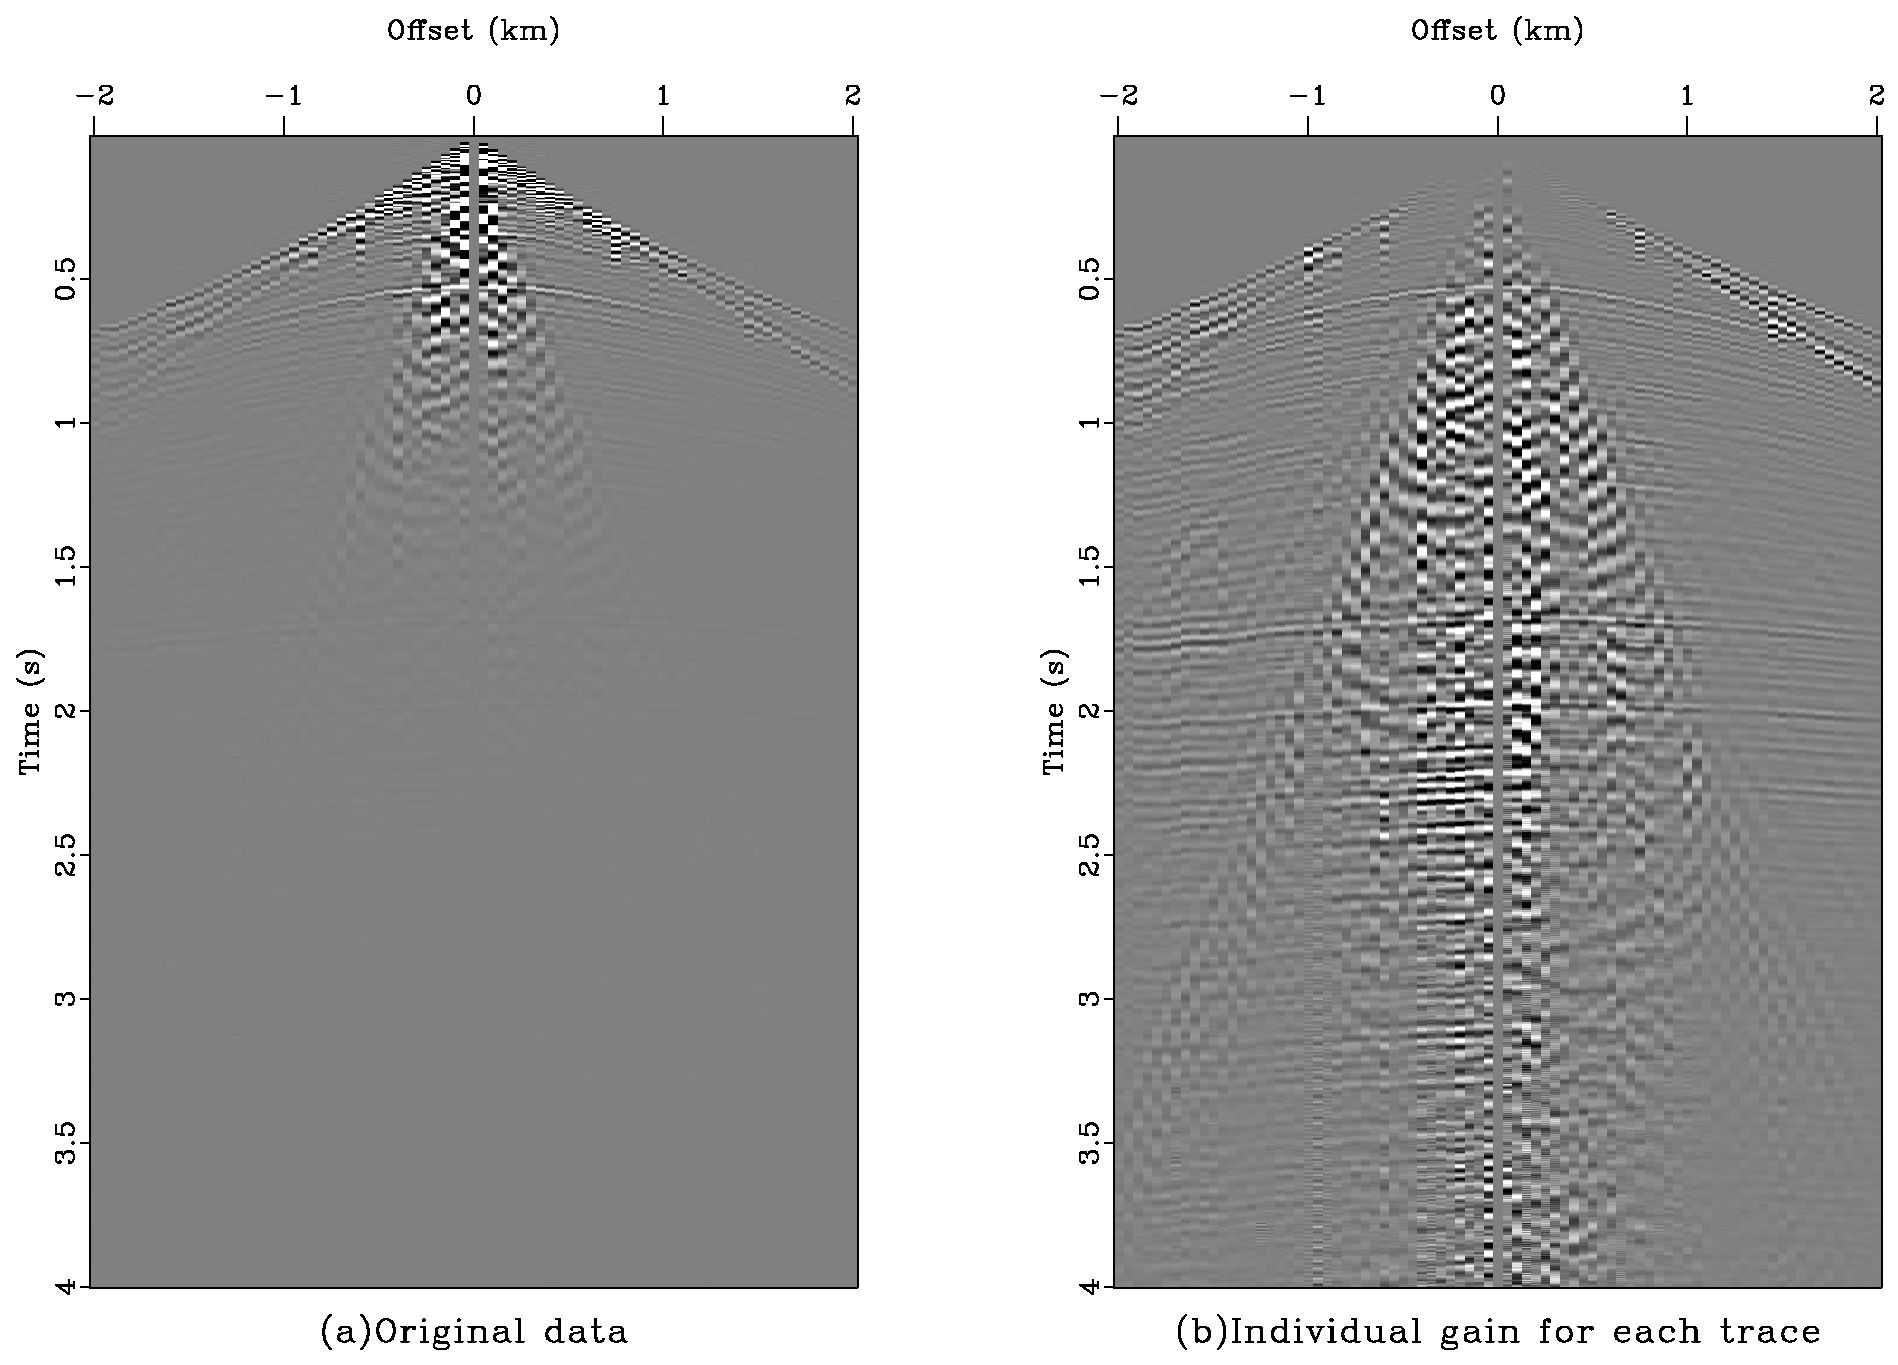
\includegraphics[width=0.5\textwidth]{individual_gain_data_by_trace_time_sidebyside.pdf}
    \caption{Comparison of original shot record and shot record where each trace was gained individually using median balancing.}
    \label{fig:shot_individual_gained}
\end{figure}

\begin{figure}[h]
    \centering
    \includegraphics[width=0.5\textwidth]{power_vs_traceindex_edit}
    \caption{Time power gain for each individual trace of Figure \ref{fig:shot_individual_gained}b.}
    \label{fig:power_vs_traceindex}
\end{figure}

\begin{figure}[h]
    \centering
    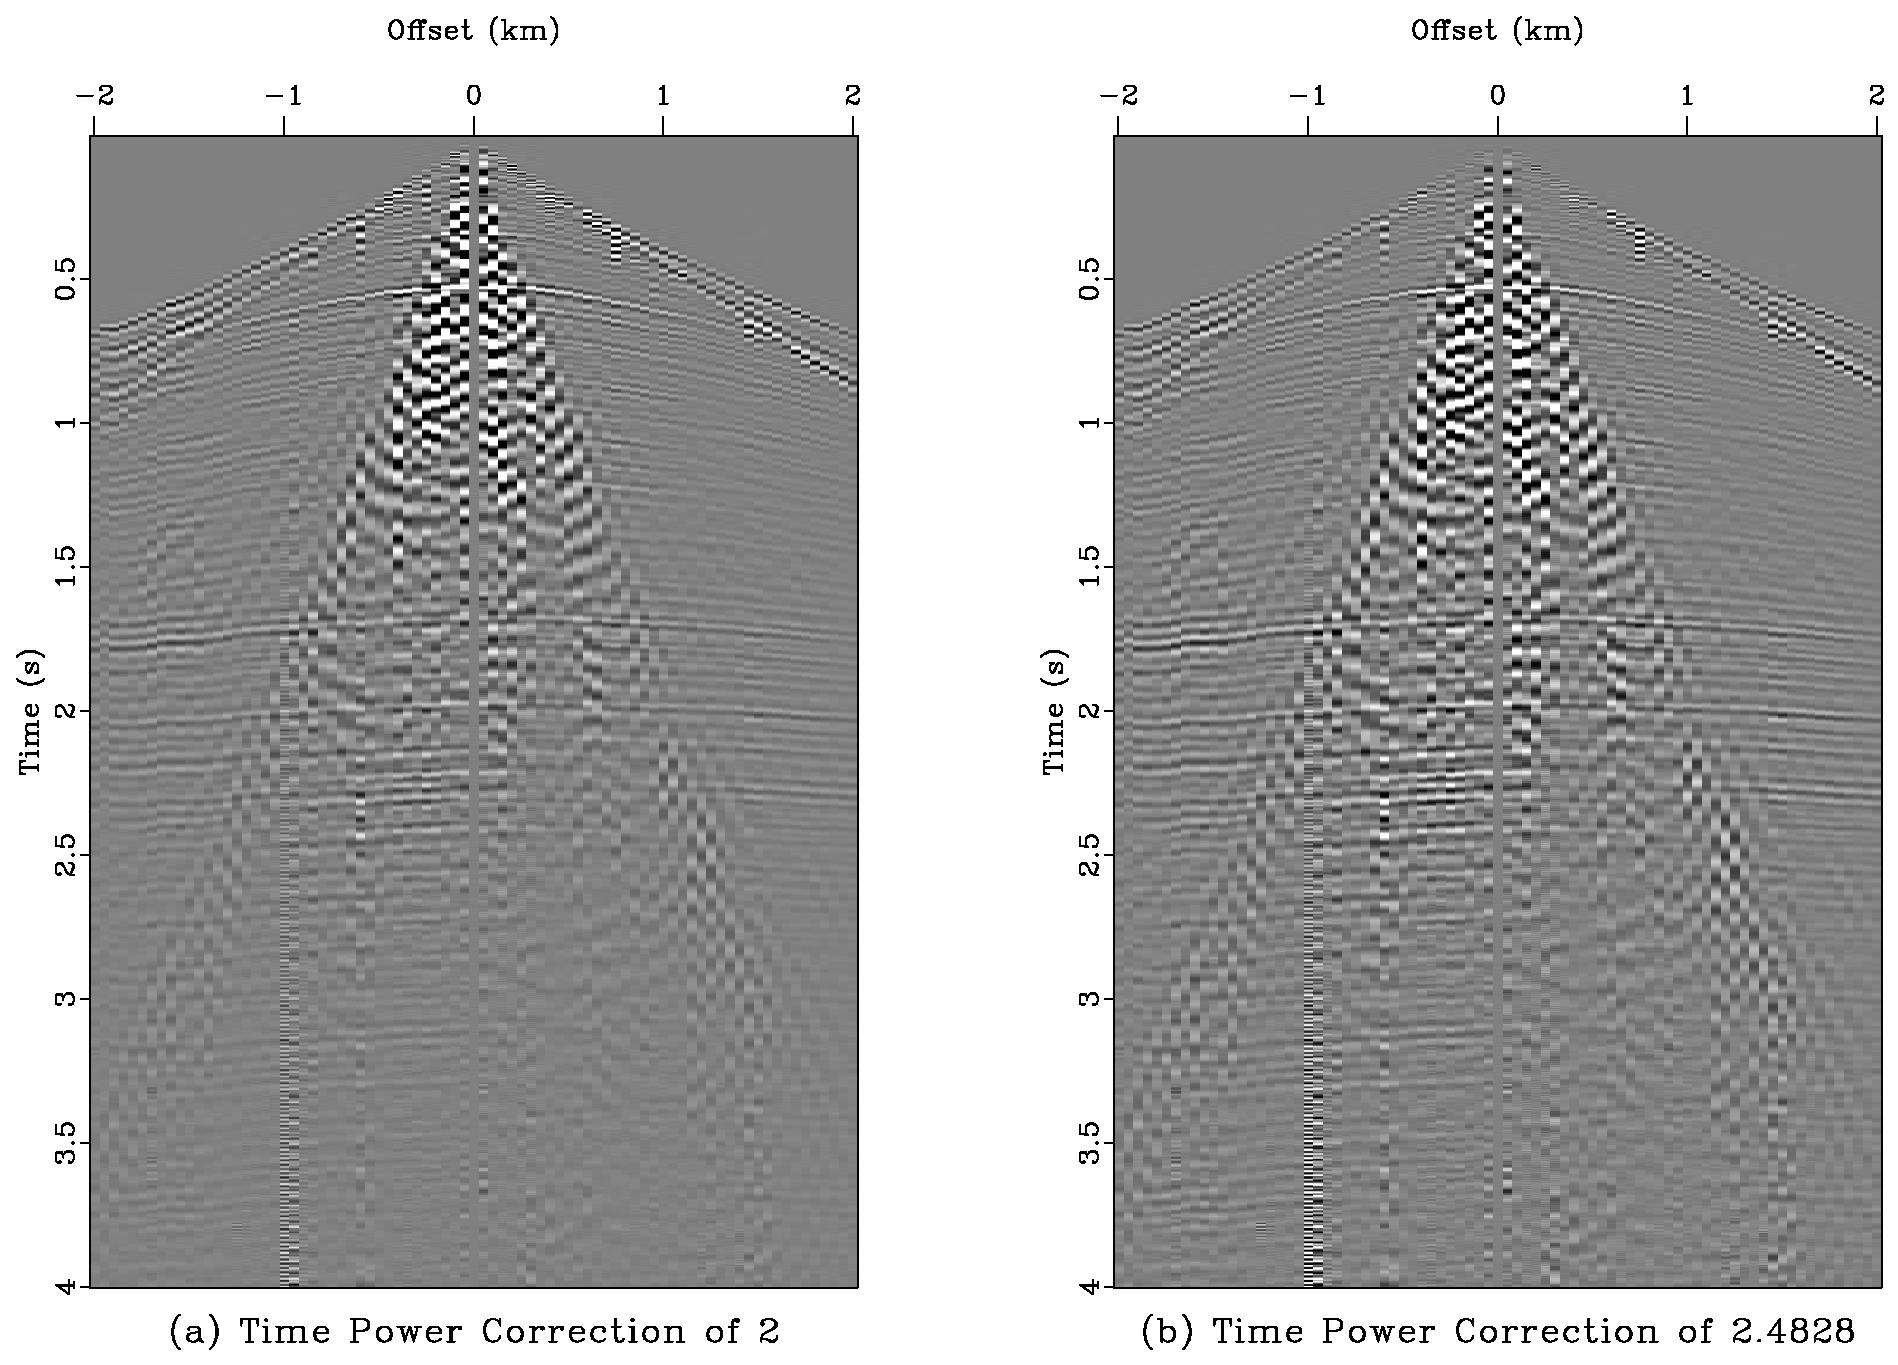
\includegraphics[width=0.5\textwidth]{original_data_sidebyside.pdf}
    \caption{Comparison when data is gained with fixed $\gamma$ power for each trace. The first gain is set at $\gamma=2$ and the second gain of $\gamma=2.4828$ was discovered via median balancing. }
    \label{fig:shot_family_gained}
\end{figure}



%\begin{figure}[h]
%    \centering
%    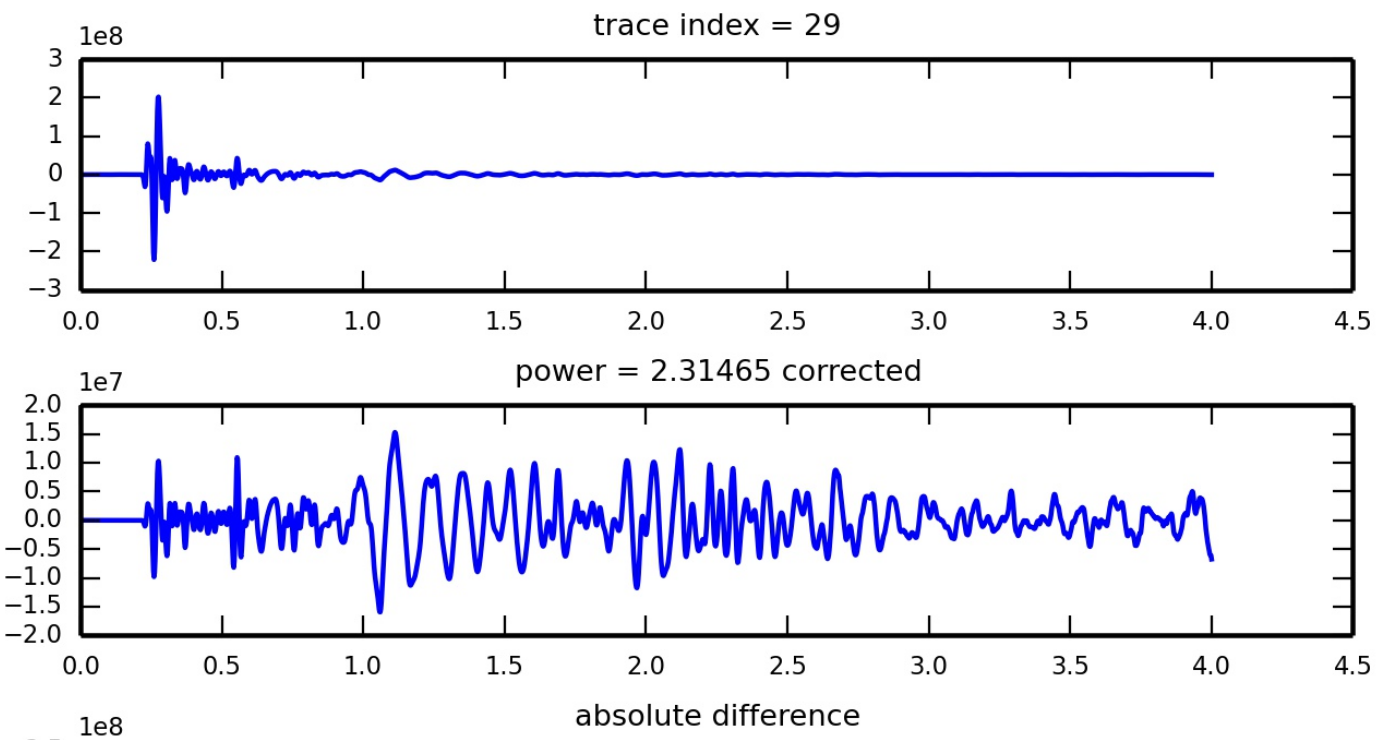
\includegraphics[width=0.5\textwidth]{trace29}
%    \caption{Trace 29 before and after correction using individual trace median balancing.}
%    \label{fig:power_vs_traceindex}
%\end{figure}

\section{Conclusion}

We have demonstrated the usefulness of the median balancing algorithm on field data and proved a linear convergence rate guarantee under the assumption of balanced medians.  Furthermore, we showed that a certain simple structure of the signal makes the convergence rate guarantee independent of the sampling interval.

\section{ACKNOWLEDGMENTS}

We would like to thank Brittany Froese for her helpful discussions.


\onecolumn



\twocolumn

\bibliographystyle{seg}  % style file is seg.bst
\bibliography{median_balance_bib}

\end{document}
